% 2007 年四川卷理科第 6 题：球 O 及球面上的三点 A、B、C。
% 来源 PDF：gaokaomath-src/普通高考/2007/2007四川理.pdf，SHA256 6f3287a6ec1c136fb7e457cb0264d069c44eb8ff58a81cc3598f9c8f1395cc2d
% 原页：2007四川理.pdf 第 1 页（A3 三栏）第 2 栏，书页码 409，图在第 6 题选项上方。
% 重绘依据：圆表示球（半径 2），A 为上极点；赤道画成半轴 (2,0.32) 的水平椭圆，
%   后半（上弧）虚线、前半（下弧）实线，B、C 落在赤道前半弧上（B 在左、C 在右）；
%   自 A 经球面到 B、C 的两条经线按竖直投影 (sin t·cosφ, cos t+0.32·sin t·sinφ) 采样，
%   在 B、C 处切线竖直；O 到 A、B、C 的三条半径在球内，画虚线。
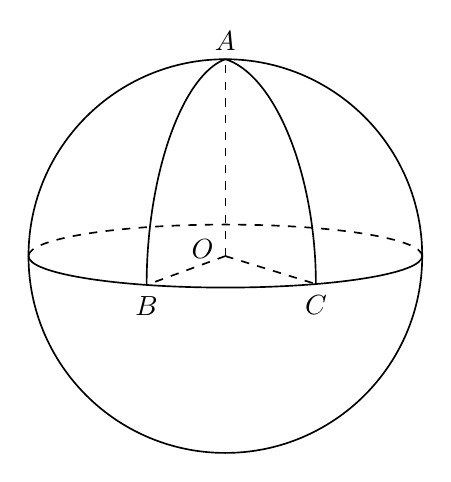
\begin{tikzpicture}[scale=1.25, semithick,
  every node/.style={inner sep=1.5pt}]
  % 球面轮廓与赤道
  \draw (0,0) circle (2);
  \draw[dashed] (2,0) arc[start angle=0, end angle=180, x radius=2, y radius=0.32];
  \draw (2,0) arc[start angle=0, end angle=-180, x radius=2, y radius=0.32];
  \coordinate (O) at (0,0);
  \coordinate (A) at (0,2);
  \coordinate (B) at (-0.800,-0.293);
  \coordinate (C) at (0.920,-0.284);
  % 球内半径（虚线）
  \draw[dashed] (O) -- (A);
  \draw[dashed] (O) -- (B);
  \draw[dashed] (O) -- (C);
  % 自 A 沿球面到 B、C 的经线弧（实线）
  \draw[domain=0:90, samples=80, smooth, variable=\t]
    plot ({2*sin(\t)*(-0.4000)},{2*cos(\t)+0.32*sin(\t)*(-0.9165)});
  \draw[domain=0:90, samples=80, smooth, variable=\t]
    plot ({2*sin(\t)*(0.4599)},{2*cos(\t)+0.32*sin(\t)*(-0.8881)});
  \node[anchor=south] at ([yshift=1pt]A) {$A$};
  \node[anchor=east] at ([xshift=-2pt,yshift=2pt]O) {$O$};
  \node[anchor=north] at ([yshift=-2pt]B) {$B$};
  \node[anchor=north] at ([yshift=-2pt]C) {$C$};
\end{tikzpicture}
